%%%%%%%%%%%%%%%%%% USAGE INSTRUCTIONS %%%%%%%%%%%%%%%%%%
% - Compile using LuaLaTeX and biber, unless there is a particular reason not to. Do not use the older LaTex/PDFLaTeX or BibTeX. (The fonts won't work correctly.)
% - Font and the report 'year' must be specified when all \documentclass or the template won't work correctly. (There's no error checking/default cases!)
% - For best performance save images/graphics as PDF files, not as png/jpg/eps. This makes no difference to how images are inserted using \includegraphics.
% - As many further packages as wanted can be loaded. Below are just an example set. Note that template itself loads a number of packages, including hyperref.
% - References are handed using biblatex.
% - Link to the presentation of theses policy: https://documents.manchester.ac.uk/DocuInfo.aspx?DocID=2863



%%%%%%%%%%%%%%%%%% META DATA SETUP %%%%%%%%%%%%%%%%%%
% This is where the document title and author are set. Other details for the title page are set later
% Note that if/when you edit these you may need to 'Recompile from scratch' to get the changes to display in the PDF. (In Overleaf, select the down arrow to the right of the 'Recompile' button)
\begin{filecontents*}{\jobname.xmpdata}
    \Title{COMP30040 Report} 
    \Author{10826115} % should be student number rather than name to help with annoymous marking
    \Language{en-GB}
    \Copyrighted{True}
    % More meta-data fielda can be added here if wanted, see https://ctan.org/pkg/pdfx?lang=en for fields
    \end{filecontents*}
    
    
    %%%%%%%%%%%%%%%%%% DOCUMENT SETUP %%%%%%%%%%%%%%%%%%
    \documentclass{uom_eee_dissertation_casson} 
    
    
    %%%%%%%%%%%%%%%%%% PACKAGES AND COMMANDS %%%%%%%%%%%%%%%%%%
    
    % Packages
    \usepackage{graphicx,psfrag,color} % for postscript graphics files
    \graphicspath{ {./images/} }
    \usepackage{amsmath}               % assumes amsmath package installed
    \allowdisplaybreaks[1]           % allow eqnarrays to break across pages
    \usepackage{amssymb}               % assumes amsmath package installed 
    \usepackage{url}                   % format hyperlinks correctly
    \usepackage{rotating}              % allow portrait figures and tables
    \usepackage{multirow}              % allows merging of rows in tables
    \usepackage{lscape}                % allows pages to be typeset in landscape mode
    \usepackage{tabularx}              % allows fixed width tables
    \usepackage{verbatim}              % enhanced version of built-in verbatim environment
    \usepackage{footnote}              % allows more control over footnote environments
    \usepackage{float}                 % allows H option on floats to force here placement
    \usepackage{booktabs}              % improve table line spacing
    \usepackage{lipsum}                % for adding dummy text here
    \usepackage[base]{babel}           % for proper hypthenation in lipsum sections
    \usepackage{subcaption}            % for multiple sub-figures in a single float
    % Add your packages here
    
    % Optional: for adding alt-text to images:
    %\usepackage{pdfcomment}            % for alt text for accessibility
    % Then to add images use:
    % \pdftooltip{\includegraphics[width=0.5\textwidth]{image.pdf}}{Alt-text here}
    % This makes the text in the image non-select-able though (assuming it's a vector file)
    
    % Custom commands
    \newcommand{\degree}{\ensuremath{^\circ}}
    \newcommand{\sus}[1]{$^{\mbox{\scriptsize #1}}$} % superscript in text (e.g. 1st)
    \newcommand{\sub}[1]{$_{\mbox{\scriptsize #1}}$} % subscript in text
    \newcommand{\sect}[1]{Section~\ref{#1}}
    \newcommand{\fig}[1]{Fig.~\ref{#1}}
    \newcommand{\tab}[1]{Table~\ref{#1}}
    \newcommand{\equ}[1]{(\ref{#1})}
    \newcommand{\appx}[1]{Appendix~\ref{#1}}
    
    
    
    %%%%%%%%%%%%%%%%%% REFERENCES SETUP %%%%%%%%%%%%%%%%%%
    
    % Setup your references here. Change the reference style here if wanted
    \usepackage[style=ieee,backend=biber,backref=true,hyperref=auto]{biblatex}
    % Note backref=true adds a page number (and hyperlink) to each reference so you can easily go back from the references to the main document. You may prefer backref=false if you need to stick strictly to a given reference style
    
    
    % Fixes which can't be applied in the .cls file
    \DefineBibliographyStrings{english}{backrefpage = {cited on p\adddot},  backrefpages = {cited on pp\adddot}}
    %  \renewcommand*{\bibfont}{\large}
    
    
    % Add more .bib files here if wanted
    \addbibresource{references.bib}
    
    
    
    %%%%%%%%%%%%%%%%%% CUSTOM MODIFICATIONS %%%%%%%%%%%%%%%%%%
    \usepackage{xcolor}
    % Define a custom quote environment
    \renewenvironment{quote}
    {
    \par\setlength{\leftskip}{10pt}
    \begin{tabular}{|p{0.9\linewidth}}  % Vertical bar on the left
    \setlength{\leftskip}{10pt}
    \itshape
    }
    {
    \end{tabular}
    \par
    }
    
    %%%%%%%%%%%%%%%%%% START DOCUMENT %%%%%%%%%%%%%%%%%%
    
    % Don't edit these lines, title and author are automatically taken from the document meta-data defined above
    \begin{document}
    \makeatletter
    \title{\xmp@Title}
    \studentid{\xmp@Author}
    \makeatother
    
    % Set the below yourself
    \course{Computer Science}  % "Master of Science in" is added automatically
                                                     % Our courses are: Advanced Control and Systems Engineering, Advanced Control and Systems Engineering with Extended Research, Communications and Signal Processing, Communications and Signal Processing with Extended Research, Electrical Power Systems Engineering, Advanced Electrical Power Systems Engineering, Renewable Energy and Clean Technology, Renewable Energy and Clean Technology with Extended Research
    \submitdate{2025}                                  % regulations ask only for the year, not month
    \wordcount{TODO}		                           % use \wordcount{} to set the count, \thewordcount to print in the text
    \maketitle
    
    
    %%%%%%%%%%%%%%%%%% LISTS OF CONTENT %%%%%%%%%%%%%%%%%%
    \uomtoc
    % other lists are not required, but can include \uomlof and \uomlot if really want to
    \uomlof
    \uomlot
    
    %%%%%%%%%%%%%%%%%% ABBREVIATIONS %%%%%%%%%%%%%%%%%%%%%
    \phantomsection\addcontentsline{toc}{section}{Abbreviations and Acronyms}
    \section*{Abbreviations and Acronyms}
      % ALWAYS define abbreviations on first use
    
      \begin{description}
        \item[AI] Artificial Intelligence
        \item[API] Application Programming Interface
        \item[CD] Compact Disc
        \item[CDPA] Copyright, Designs and Patents Act 1988
        \item[CNN] Convolutional Neural Network
        \item[OCR] Optical Character Recognition
        \item[ML] Machine Learning
        \item[ToS] Terms of Service
        \item[TOU] Terms of Use
        \item[UX] User Experience
      \end{description}
    
    %%%%%%%%%%%%%%%%%% ABSTRACT %%%%%%%%%%%%%%%%%%%%%%%%%%
    \begin{abstract} % put abstract here. Limit is 1 page.
      Vinyl is back!
    
    \end{abstract}%
    \clearpage
    
    
    
    %%%%%%%%%%%%%%%%%% DECLARATIONS %%%%%%%%%%%%%%%%%%
    \uomdeclarations % Don't need unless final thesis
    
    
    
    %%%%%%%%%%%%%%%%%% ACKNOWLEDGEMENTS %%%%%%%%%%%%%%%%%%
    \begin{uomacknowledgements}
    I would like to extend my gratitude to the noble mahogany tree, whose sacrifice provided not only the material for a Welsh love spoon - by which I proposed and became engaged to my beloved fiancée - but also the offcuts that found purpose in the physical interface of this project. Your contribution to both my personal and academic life has been truly invaluable.
    
    Also, to my close friend Joshua Bond’s dissertation \cite{jdbond}, which I have yet to fully read- but I am sure it is great.
    \end{uomacknowledgements}
    
    
    
    %%%%%%%%%%%%%%%%%% SECTION 1 %%%%%%%%%%%%%%%%%%
    \section{Introduction}
    
      % Written by **Sean Bechhofer**: https://studentnet.cs.manchester.ac.uk/ugt/year3/project/projectbookdetails.php?projectid=55259
    
      % Vinyl is back! According to the [NME](https://www.nme.com/news/music/uk-vinyl-sales-2023-reach-highest-level-since-1990-3563676), UK sales of vinyl in 2023 were the highest seen since 1990. Vinyl has always remained popular among niche genres, but we are also seeing mainstream artists like Taylor Swift and Lana Del Ray releasing, and selling large volumes of albums on the format. Vinyl records have also recently been added in to the ONS "Basket of Goods and Services": a carefully selected set of items representative of the goods and services that UK consumers typically spend their money on ([ONS](https://www.ons.gov.uk/news/news/arecordrevivalthatscookingupastormvinylmusicandairfryersspintheirwayintothebasketofgoods)).
    
      % Fans of the format claim better sound reproduction, with a fuller frequency range and a "warmth" lacking in digital formats such as CD. Playing vinyl requires specialist equipment: while the ritual of putting a disc on the turntable and dropping the needle is, for some, part of the experience, it can also be seen as an inconvenience.
    
      % The aim of this project will be to develop an application that supports a blending of the physical and digital worlds. A physical artefact such as an LP is scanned using a camera. The information on the label or cover is then used to identify the release which can be played. This content could be retrieved from a streaming service such as Spotify or Apple Music, an artist site such as Bandcamp [Bandcamp](https://bandcamp.com/), or the user's own personal media library. This would then allow a user to "play" their records without a turntable. Although the audio quality may not match that of vinyl, such an application would appeal to those who like to collect vinyl for its own sake, or who appreciate the larger format artwork that comes with an old school LP. The application could run on a mobile phone or specialist hardware such as a Raspberry Pi equipped with a camera.
      % Example methods that could be used for identification of the release include bar codes, QR codes or OCR acting on label text.
    
      % For a stretch goal, the application could be extended to cover other media: the cassette tape ([Guardian](https://www.theguardian.com/music/2023/apr/20/fun-way-consume-music-why-sales-of-cassette-tapes-soaring)) is also experiencing a come back, although the [eight-track](https://en.wikipedia.org/wiki/8-track_cartridge) is unlikely to be retrieved from the dustbin of history.
      % The project should be considered as challenging. It will require integration of several technologies and some creativity.
    
    \subsection{Background and motivation}
    
    \subsection{Aims and objectives}
    
    % PROJECT PLAN?
    
    \subsection{Report structure} % ROADMAP
    
      This report consists of seven chapters:
      \begin{description}
      \item[Chapter 1] presents an introduction to the project.
      \item[Chapter 2] presents the background behind this project, ...
      \item[Chapter 3] presents details on the design ...
      \item[Chapter 4] presents details on the implementation ...
      \item[Chapter 5] presents the results ...
      \item[Chapter 6] presents an evaluation  ...
      \item[Chapter 7] presents a discussion of the conclusion, limitations, and possible improvements of the project.
    \end{description}
    
    
    %%%%%%%%%%%%%%%%%% SECTION 2 %%%%%%%%%%%%%%%%%%
    \section{Background and Literature Review} % LITERATURE REVIEW / BACKGROUND
      % [ ] summary of similar systems
      % [ ] explanations of concepts relied on later
      % [ ] advanatges and disadvantages of approaches
      % [ ] highlight problems I will improve
      % [ ] cite all references
    
      \subsection{Overview of Related Systems}
    
        Whilst the creation of a digitised turntable software is a rather novel idea, it is important to consider where this sits in the existing landscape, to understand important technologies and design decisions used in similar projects, to best utilise them.
      
        \subsubsection{Vinyl Systems}
            % Research into questions such as 'why do people like vinyl so much?' and 'why is it making a comeback?'. Traits distilled from this feed into later design choices (I have chosen to make a make a physical artefact with a mahogany base, because physicality and aesthetics are important the people who would potentially use this system).
    
            \begin{quote}
                ``Vinyl is back!'' \cite{bechhofervttspec}
            \end{quote}
            
            In 2023, vinyl sales in the UK reached their highest level since 1990 \cite{geraghty2023uk_vinyl_sales}, indicating a continued growth in the ``vinyl revival'' \cite{vinylRevival} (see Figure~\ref{fig:vinyl_sales}), indicating that this trend is not the short-term fad that it was commonly thought to be when it first started in 2008-2009.
            
            \begin{figure}[htbp]
                \centering
                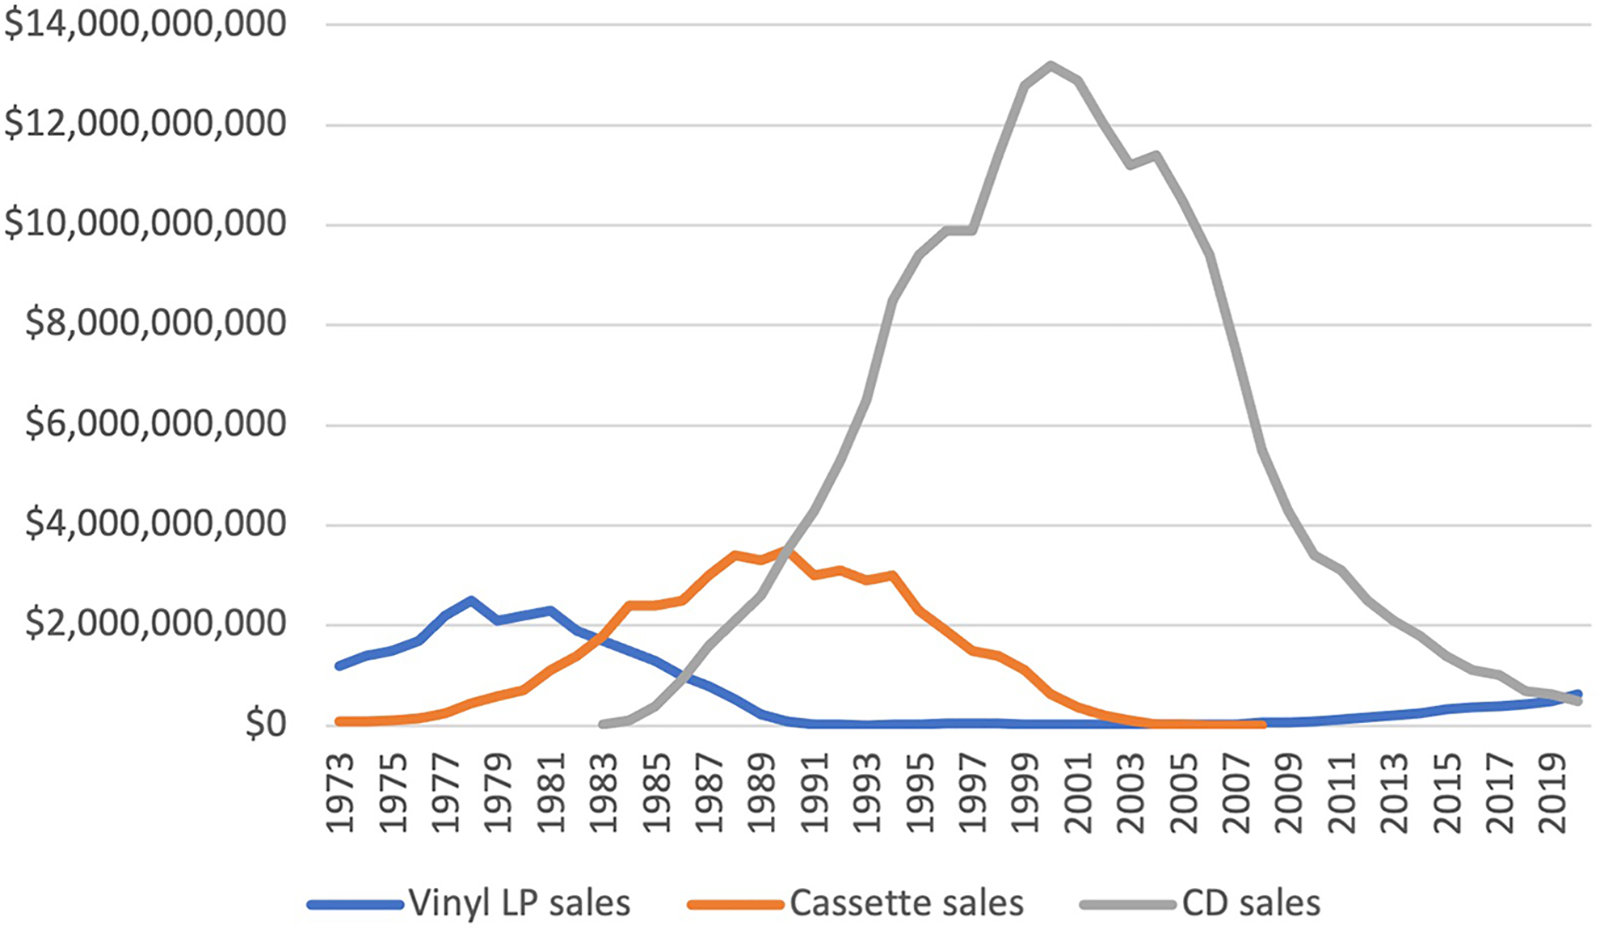
\includegraphics[width=\linewidth]{images/vinyl_sales_2023.png}
                \caption{Vinyl LP, Cassette, and CD Sales Revenue (1973–2020) \cite{vinylRevival}.}
                \label{fig:vinyl_sales}
            \end{figure}
    
            The continuation of this trend suggests a resurgence in physical music formats, and understanding why this came about, as well as why it has not died out, is important to consider for this project, particularly from a UX perspective. This is especially true, as vinyl collector form a large part of the potential audience for such a product.
    
            Whilst it is now taken for granted, records at the time, (and their predecessors: Edison's cylinder recordings), were a revolutionary introduction to the world of music. Prior to this point, music was very much a temporal and localised art-form, which, unlike their visual counterparts could not be stored, transported, or reproduced- even if a song could be transcribed into musical notes, any one performance could never again be heard once it had completed. That is, until the recording medium became available on mass to the public.
    
            % Aesthetics
            \paragraph{Aesthetics and Emotions}
                % nostalgia
                % vibes
    
            % Audiophiles
            \paragraph{Audiophilia and Quality} // temp % not sure why this spacing breaks without this
    
                \begin{quote}
                    \textbf{audiophile}: a person who is especially interested in high-fidelity sound reproduction. \cite{audiophile2025}
                \end{quote}
    
                % quality
          
              % Ownership
              % Physicality
            \paragraph{Physicality and Ownership}
    
                In today's digital day and age, ownership is becoming an important matter for consumers. Unlike with physical copies of media, digital versions offered by vendors are tenuously offered to users. These offering often come with the fine-print of being merely revocable \cite{polygon2024cartoon_network_delisting} licenses when purchased, instead of consumer ownership \cite{verge2024steam_license}. This transition has upset many people, with there being many calls to bring back genuine ownership \cite{stanton2024gamers_pushback}, with legislation even being passed in California to make this fact more transparent to consumers \cite{california2024ab2426}.
    
                This sentiment extends just beyond games, and applies also to music. If someone's streaming service of choice stops serving a particular piece of music that they want, then they are currently powerless to do anything to prevent this. If they, however, own the physical discs or digital audio files, then they can ensure that they can listen to said audio, regardless of whatever licensing disputes may lead to the removal of digital media (see \cite{bains2022lotr_strategy}).
    
                There are also concerns that some music streaming surfaces do not proportionately pay artists for their work, yet, most artists have no choice but to just accept this, as the newfound convenience of streaming makes sales and exposure very difficult for new artists. Because of this, many consumers still purchase physical media, even if they also use a streaming service, purely to ensure that the artists they like are being fairly supported.
    
                Therefore, a system can benefit from helping users permanent access to their tracks, perhaps by making use of local audio files and therefore offering the safety of available. Additionally, creating a system that marries the physical and digital worlds of music could be beneficial for people who collect physical copies of albums in addition to having digital access through a service or local files, and could be seen as a gateway of the digital continence, whilst still satisfying and even endorsing the ethical desire to purchase music directly from an artist's label.
    
        \subsubsection{Image Recognition}
    
            Image recognition is is the creation of software and tools which can be used to identify objects, places, people, etc. in digital images, which arguably does not predate 1946 \cite{hall1979computer}. However, in this brief time, the field has undergone several drastic changes as technology has advanced \cite{imagenetclasscnn}, and is still be redefined in the present day, particularly with the arrival of machine learning approaches, with new implementations being utilised across the field (e.g., \cite{RAMPRASAD2025100556}, 2025).
            
            \paragraph{Traditional Methods}
    
                Some stuff.
            
            \paragraph{Emergence of Convolutional Neural Networks}
    
                Some more stuff.
    
        \subsection{Legal and Ethical Considerations}
    
          The training and use of machine learning models for image classification requires the acquisition and processing of data, which, in order to effectively handle the cover art of existing albums, necessitates obtaining and using their copyrighted artworks. This raises both legal and ethical concerns, particularly regarding compliance with UK copyright law and exemptions. This section examines the legal basis for dataset usage, fair dealing exemptions, and the ethical implications of using copyrighted material in an academic AI project.
    
              \subsubsection{Copyright Law and Fair Dealing}
                  % explain copyright law
                  Under the \textit{Copyright, Designs and Patents Act 1988} \cite{cdpa1988}, creative works, including album covers, are protected from unauthorised use, reproduction, distribution, and modification.
          
                  % introduce fair dealing
                  However, UK law also provides a key exception known as Fair Dealing, which allows limited use of copyrighted material under specific conditions, although such exemptions are only granted under very specific circumstances and for a very limited scope of use. Importantly, it is not a rigid rule but a context-dependent legal doctrine, evaluated on a case-by-case basis. The law does not explicitly define what qualifies as fair dealing; instead, courts assess whether a use is reasonable and justified based on the combination of several established legal factors.
                  
                  One of the most relevant exemptions is non-commercial research, as outlined in \textit{Section 29(1)} of the CDPA:
                  \begin{quote}
                      Fair dealing with a work for the purposes of research for a non-commercial purpose does not infringe any copyright in the work provided that it is accompanied by a sufficient acknowledgement. \cite{cdpa1988}
                  \end{quote}
    
                  This indicates that non-commercial academic research can be exempt from copyright infringement if proper attribution is provided. However, the applicability of this exemption depends on further and additional factors, such as the amount of material used and its impact on the copyright holder’s market.
    
              % 1. Using a dataset to create a model
              \subsubsection{Use of Artworks in Model Training}
              
                  Album covers are protected by copyright as highly creative works. Any reproduction or modification is typically restricted without permission from the copyright holder. As such, the bar needed for fair dealings is very high when dealing with such artwork. However, training a classification model may qualify for fair dealing, provided certain conditions are met.
    
                  A key legal question is whether machine learning training qualifies as ``\textit{computational analysis}'' under \textit{Section 29A} of the CDPA, which states:
                  \begin{quote}
                      (1) The making of a copy of a work by a person who has lawful access to the work does not infringe copyright in the work provided that—
                  
                          (a) the copy is made in order that a person who has lawful access to the work may carry out a computational analysis of anything recorded in the work for the sole purpose of research for a non-commercial purpose, and
                          
                          (b) the copy is accompanied by a sufficient acknowledgement (unless this would be impossible for reasons of practicality or otherwise). \cite{cdpa1988}
                  \end{quote}
    
                  This expresses that there is a strong argument for legal use of copyrighted materials in creating a computational model which classifies data by comparisons of analytically-derived embeddings.
    
                  It is, however, important to consider whether image processing qualifies as analysis under this law or whether this interpretation is too broad, given that past applications of computational analysis have predominantly involved text, and that image processing of this kind is still relatively new. Since there is no clear legal precedent on this specific topic (with changes being in the process of being made \cite{guardian2024uk_ai_copyright}), further legal clarification over the next few years will be necessary to definitively confirm or deny its applicability to image-based AI models. But, in the time before then, it can be used as a basis.
    
                  It also reiterates the need for attribution, but, notably states that this is only required in cases where it is feasibly practical.
    
                  Given these factors, classification likely qualifies under Fair Dealing because the model does not generate new images but merely classifies existing ones. This distinction is important, especially given recent legal scrutiny of generative AI models like OpenAI’s \textit{DALL·E} \cite{times2025christies_ai_auction}\cite{guardian2025ai_art_auction}, which create derivative works rather than merely labelling.
    
                  None of this is clear-cut, however, as we are still in an uncertain time with the law not having been stabalised after the emergence and mass adoption \cite{bick2024rapid} of these new technologies. It is worth noting, however, that there are currently proposals for UK law the explcitly allow the use of copyrighted materials in such cases \cite{guardian2024uk_ai_copyright}, whereas, in the US, there is starting to be legal prescendent of cases winning on the basis \cite{apnews2025thomson_reuters_ai_case} of AI agents using copyrighted data.
    
              % 2. Sourcing said dataset
              \subsubsection{Legal Compliance in Dataset Sourcing}
    
                  Beyond Fair Dealing considerations, data sourcing must be legally compliant. According to \textit{Section 29A} \cite{cdpa1988}, only individuals with lawful access to copyrighted works may use them for computational analysis. Therefore, it is essential to determine how these images can be legitimately acquired.
    
                  Machine learning models must fully process training images in their entirety to generate a model. This requires the whole image to be either stored persistently (on disk) or temporarily (in memory). Even if the image is only ever stored and processed in chunks (similar to how streaming providers serve video data), the overall image is eventually processed by the model. \textit{Section 28A} outlines more leniency for cases where only temporary copies are stored, for lawful access.
    
                  It is also important to consider if entire images are required, as opposed to only sections of them. If it would be possible to achieve the desired result using only subsets of the acquired dataset, then more data would be stored and used than is justified. The legal precedent \textit{Ashdown v Telegraph Group Ltd (2002)}, highlights that:
    
                  \begin{quote}
                      The third most important factor is the amount and importance of the work that has been taken . . . in some circumstances the taking of an excessive amount, or the taking of even a small amount if on a regular basis, would negative fair dealing. \cite{tmlocad}
                  \end{quote}
    
                  Thus, ensuring only necessary data is used is critical for compliance.
    
                  % 3. ToS compliance
                  In addition to just the handling of the data, however, its source must also be considered. There are three methods by which the training dataset could be acquired: by fetching data from an API, by scraping the data from the web, or, by manually taking the required photos (either by just me, personally, or by crowd-sourcing the images). Realistically, the first two options are most practically feasible.
    
                  There are many vendors of the cover arts of music albums. Notably, music vendors (such as \textit{Spotify}) and music collection and review sites (such as \textit{Discogs}) provide the album arts in a structured format where the artworks are synchronised with the albums which they belong to. However, due to the recent boom of generative AI models - and the controversy surrounding them \cite{apnews2025mccartney_ai_warning} - many vendors have explicitly prohibited the use of their data for machine learning in their Terms of Services.
    
                  % specific examples should probably be discussed under 'Design'
                  \begin{quote}
                      Do not use the Spotify Platform or any Spotify Content to train a machine learning or AI model or otherwise ingest Spotify Content into a machine learning or AI model.
                  \end{quote} \cite{spotifyDevPolicy} (III.14)
                  \begin{quote}
                      Do not misuse the Spotify Platform, including by i. using the Spotify Platform or any Spotify Content to train a machine learning or AI model or otherwise ingesting Spotify Content into a machine learning or AI model;
                  \end{quote} \cite{spotifyDevTerms} (IV.2.a.i)
                  \begin{quote}
                      [Discogs] strictly prohibit (1) the development of any software program, including, but not limited to, training a machine learning or artificial intelligence (AI) system using the Service content
                  \end{quote} \cite{discogsToS} (LICENSE AND SITE ACCESS)
    
                  However, if a site has more permissive policies, allowing the training of AI models, then, as long as the images are handled appropriately, they can be lawfully accessed and used.
    
              \subsubsection{Ethical Considerations}
              % Even if it's legally permissible, is it ethically responsible?
              % Does it impact the commercial success of artists?
              % Transparency & attribution concerns.
    
                  Even if it is legally permissible to source and use these images, it is also important to consider whether or not it is ethically responsible. These images, at the end of the day, are the highly creative works of artists, whose livelihoods come from their creations \cite{heikkila2022ai_art}. Reproducing (by downloading) and using their works therefore cannot be done without serious moral consideration.
    
                  Most significantly, it is worth noting that this AI model is not generative (which is where most of the recent controversies stem from \cite{apnews2025mccartney_ai_warning}), and therefore, instead of producing its own artworks based off of the images fed to it, it simply classifies them by labelling them with its prediction of their corresponding album. Therefore, whilst the model is technical derived from the artist's works, the produced work is not in competition with the additional artists - unlike generative agents \cite{times2025photographer_ai_copy} - and therefore should not have a negative impact on their commercial success. If anything, it is argued that this system should benefit them, by encouraging the purchasing of physical media, and garnering instances of playing their content on a revenue-generating service.
    
                  Furthermore, as this does not share or distribute the images themselves with the users, I believe it to be even more safe, as the only artefact generated from these images are a classification system which can be used by the user, but even the numerics themselves are not made accessible to the user.
    
                  And, whilst the law allows for the exclusion for explicit attribution of all involved copyright holders, this may not be ethical. However, as this is a classification system, it arguably gives some degree of implicit accreditation to the artworks used in the training process, when the predicted label is used to redirect the user to said album.
    
              \subsubsection{Conclusion}
    
                  This section examined the legal and ethical implications of using copyrighted album covers in machine learning. Based on UK Fair Dealing exemptions in the CDPA 1988, I would argue that there is a solid grounding this project likely qualifies as a legally permissible use case, provided:
                  \begin{description}
                      \item[-] It is a non-commercial, research project.
                      \item[-] Data is lawfully acquired from permitting sources.
                      \item[-] The dataset scale and usage is minimised to strictly what is neccessary.
                      \item[-] None of the images are shared or modified. % this will need to be checked when talking about data augmentation
                  \end{description}
                  
                  From an ethical standpoint, the project is distinguishable from controversial generative AI models, as it does not replace artists’ work or impact their revenue streams. Nonetheless, transparency and attribution best practices should be followed.
    
    %%%%%%%%%%%%%%%%%% SECTION 3 %%%%%%%%%%%%%%%%%%
    \section{Design} % DESIGN / METHODOLOGY
      What did past-Jack set out to do?
      % design diagrams!
    
      \subsection{Requirements Analysis}
          % list of requirements
    
      \subsection{System Architecture} % high-level system overview
          \subsubsection{Technology Stack}
              All of the technologies used (TS, React, bun, Python, FastAPI, etc.), and why them specifically.
    
          \subsubsection{Design Choices}
              % unique 1-1/1-many relation
              % server hardware control
              % host v. remote client
              Particular broad and niche design choices made, and why, such as:
              \begin{description}
                  \item[1.] Why use a web approach for a localised device?
                  \item[2.] Why use an unorthodox 1-1 Websocket approach for client-server calls?
              \end{description}
              Also things such as 'point of truth handling', etc.
    
              Design philosophy of being an non-reliant on Spotify (or any other singular API) as possible
    
      \subsection{Front-end}
          \subsubsection{Primary User Interface}
              % lofi designs
    
              Minimal-UI approach \\
              Physical user interaction controls
    
          \subsubsection{Audio Playback}
              % Spotify Playback SDK
              % Spotify Web API
    
          \subsubsection{Remote Clients}
              'Remote Control' UI from an external device (mobile, etc.)
    
              Gains that this system provides: accessibility (mobility, etc), convinience, scanning of out-of-house albums, etc.
              % for convineince, the need for (33-45) adapter  can be cited
              % https://external-content.duckduckgo.com/iu/?u=https%3A%2F%2Fnotesonvinyl.com%2Fwp-content%2Fuploads%2F2022%2F04%2Fspeeds-of-the-different-record-types-1.png&f=1&nofb=1&ipt=7d1e31af8468ae7ae70f11be6bd40c897a73cf0c42aa194a5e09309f9af25945&ipo=images
              % https://external-content.duckduckgo.com/iu/?u=https%3A%2F%2Fwww.bluescentric.com%2Fimages%2Fproduct%2Flarge%2F557_2_.jpg&f=1&nofb=1&ipt=1cd939744050d9f13eb7f581b786a2f22d3787cf30dd60c2a6975a816043546f&ipo=images
      
      \subsection{Back-end}
    
          \subsubsection{Metadata Retrieval}
              % Discogs API
              % assert Discogs ToS compliance (not used for AI) 
          
          \subsubsection{Hardware Interaction}
              % RPi
      
      \subsection{Machine Learning Model Design}
          \subsubsection{Dataset Collection}
              % use of CoverArtArchive
    
          \subsubsection{Model Architecture}
    
      \subsection{Security Considerations}
          % handling of auth tokens (transient)
          % off-handing of persistence tasks
          % network hosting
          % option of same-user or any-user controls
          % API compliances
    
      \subsection{Testing Methodology}
          Design of tests and evaluations; plan for unit testing, model evaluation, etc.
    
          Does the system satisfy that physical and aesthetic desires of that the vinyl trend appeals to, whilst still offering functional convenience over original systems?
    
          \subsubsection{Validation of Effectiveness}
              1. Model performance (formal model evaluation)
              2. Usability (user feedback)
    
              3. Code robustness (Unit Tests, etc.)
    
          \subsubsection{Validation of Affectiveness}
              User feedback on aesthetics
    
    
    %%%%%%%%%%%%%%%%%% SECTION 4 %%%%%%%%%%%%%%%%%%
    \section{Implementation}
      Details realised in practice, decisions made, etc.\\
      Challenges encountered, how addressed, etc.
      % details realised in practice
      % challenges, and how overcame
      % code-level or system-specific decisions, optimizations, or trade-offs
      % integration
      \subsection{Front-end}
          \subsubsection{Challenges Encountered}
              1. Switch to minimal UI mid-production
              2. Responsive / wholeness tradeoff (do we wait for the centre label before playing the audio?)
              3. Media codec, DRM, etc. issues specific to Ubuntu/aarch64 OS.
    
      \subsection{Back-end} % maybe Front/Back should just merge to software, here
          \subsubsection{Challenges Encountered}
              1. Change of auth flow, due to 'remote client' introduction
              2. Removal of barcode detection form spec, due to camera limitations
    
      \subsection{Hardware}
          \subsubsection{Challenges Encountered}
              1. Lack of 'Measure twice, cut once' methodology (fried GPIO pin; overstrained motor driver)
              2. Voltage issues
              3. Overheating (throttling) issues
    
      \subsection{Machine Learning Model}
          \subsubsection{System Integration}
              Practice-driven discoveries, such as 'how much is not too much' when it came to model architecture and the Pi's specs.
    
          \subsubsection{Challenges Encountered}
              Internet Archive downtime!
    
    
    %%%%%%%%%%%%%%%%%% SECTION 5 %%%%%%%%%%%%%%%%%%
    \section{Results} % edit section heading as appropriate
      What was actually produced?
      % results of soft/hardware testing
      % screenshots of UI / program output
      \subsection{Software Artefact}
    
      \subsection{Hardware Artefact}
    
    %%%%%%%%%%%%%%%%%% SECTION 6 %%%%%%%%%%%%%%%%%%
    \section{Evaluation}
      % does it do what it is supposed to do?
      % how well?
      % how well against others?
      \subsection{Machine Learning Model Performance}
    
      \subsection{User Experience}
    
      \subsection{Comparison with Existing Systems}
    
      \subsection{Ethical Implications}
    
    
    %%%%%%%%%%%%%%%%%% SECTION 7 %%%%%%%%%%%%%%%%%%
    \section{Conclusions and future work} % edit section heading as appropriate
      \subsection{Conclusions}
          % summarise results
          % achieved aims?
          % improvements!
      
      \subsection{Future work}
          % ideas for further work
          % big ideas; what could be done with my project?
    
    
    %%%%%%%%%%%%%%%%%% REFERENCES %%%%%%%%%%%%%%%%%%
    %\clearpage % uncomment to start on a new page if wanted
    \printbibliography[title={References},heading=bibintoc] % a single list of references for the whole thesis
    
    
    
    %%%%%%%%%%%%%%%%%% APPENDICES %%%%%%%%%%%%%%%%%%
    \begin{uomappendix} 
      % screen dumps of UI
      % important but large results
      \section{Project outline}
      Project outline as submitted at the start of the project is a required appendix. Put here. 
      
      \section{Risk assessment}
      Risk assessment is a required appendix. Put here.
      
      %\section{Other appendices as necessary}
    \end{uomappendix}
    
    
    %%%%%%%%%%%%%%%%%% END MATTER %%%%%%%%%%%%%%%%%%
    \end{document}